\chapter{Appendix B: Simulation a-3b-256} 

Simulation a-3b-256 has the exact same optimization problem parameters as simulation 
a-3b (Table \ref{tab:simulationa3b}) except for an increase in population size to 256
individuals. 
Table \ref{tab:a3b-256-hypervolume} shows the hypervolume value at each generation, 
confirming that simulation a-3b-256 converges by generation 4. 
\begin{table}[htbp!]
    \centering
    \onehalfspacing
    \caption{Simulation a-3b-256 hypervolume values at each generation.}
	\label{tab:a3b-256-hypervolume}
    \footnotesize
    \begin{tabular}{ll}
    \hline 
    \multicolumn{2}{c}{\textbf{Three Objectives: Simulation a-3b-256}} \\
    \multicolumn{2}{c}{Reference point: (0.07, 1700, 1.8)} \\
    \hline 
    \textbf{Generation} & \textbf{Hypervolume [-]} \\
    \hline
    1 & 5.7867 \\
    2 & 5.8019 \\
    3 & 5.9412 \\
    4 & 5.9675 \\
    \hline
    \end{tabular}
\end{table}
Figure \ref{fig:assem-obj-3-all-256-2d} shows a plot of the final generation's reactor 
models' $PF_{total}$ against $T_{max}$ against $PPF_{fuel}$; crosses mark the reactor 
models that fall on the Pareto front.
Figure \ref{fig:assem-obj-3-all-256-distr} shows the 38 TRISO packing fraction 
distributions in the final generation, labeled numerically, that fall on the 
Pareto front. 
\begin{figure}[htbp!]
    \begin{subfigure}{\textwidth}
        \centering
        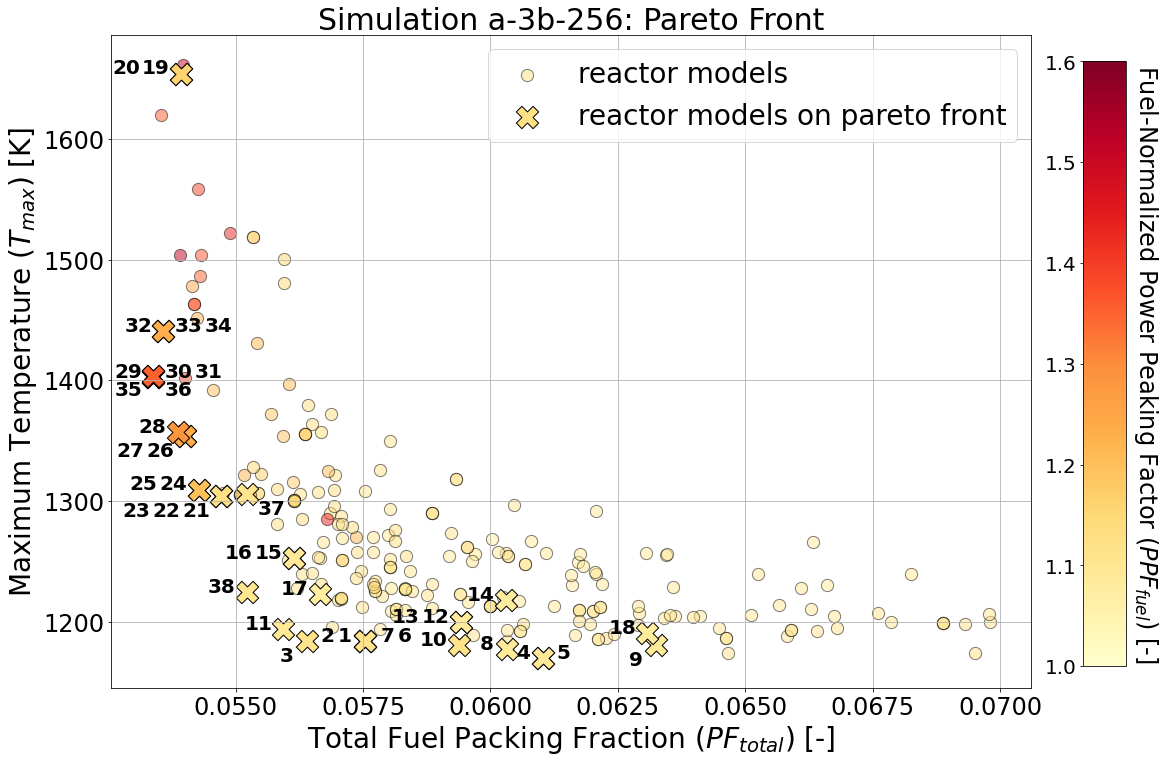
\includegraphics[width=\linewidth]{assem-obj-3-all-256-2d.png}
        \caption{Plot of final generation's reactor models' $PF_{total}$ against 
        $T_{max}$ against $PPF_{fuel}$ as a color dimension. 
        Crosses indicate the reactor models on the 
        Pareto front. Cross numbering correspond to TRISO distributions in Figure 
        \ref{fig:assem-obj-3-all-distr}.}
        \label{fig:assem-obj-3-all-256-2d} 
    \end{subfigure}
    \caption{Simulation a-3b-256 -- ROLLO triple-objective optimization with 
    256 population size to minimize total fuel packing fraction ($PF_{total}$), 
    maximum temperature ($T_{max}$), and fuel-normalized power peaking factor 
    ($PPF_{fuel}$) in the one-third assembly. 
    Input parameters varied: total fuel packing fraction $PF_{total}$, 
    TRISO packing fraction distribution ($\rho_{TRISO}(\vec{r})$), 
    coolant channel shape $(r_1, r_2, r_3, r_4, r_5)$.}
    \label{fig:assem-obj-3-all-256}
\end{figure}
\begin{figure}[htbp!]
    \ContinuedFloat
    \begin{subfigure}{\textwidth}
        \centering
        \includegraphics[width=\linewidth]{assem-obj-3-all-256-distr.png}
        \caption{TRISO distributions for the 38 reactor models on the Pareto front.
        Numbered reactor models correspond to numbered crosses in Figure 
        \ref{fig:assem-obj-3-all-256-2d}. 
        Note that some models have identical distributions, resulting in the 23 plots 
        in this subfigure.}
        \label{fig:assem-obj-3-all-256-distr} 
    \end{subfigure}
    \caption{(contd.) Simulation a-3b-256 -- ROLLO triple-objective optimization with 
    256 population size to minimize total fuel packing fraction ($PF_{total}$), 
    maximum temperature ($T_{max}$), and fuel-normalized power peaking factor 
    ($PPF_{fuel}$) in the one-third assembly. 
    Input parameters varied: total fuel packing fraction $PF_{total}$, 
    TRISO packing fraction distribution ($\rho_{TRISO}(\vec{r})$), 
    coolant channel shape $(r_1, r_2, r_3, r_4, r_5)$.}
\end{figure}

Figure \ref{fig:assem-obj-3-all-256} demonstrates that \gls{ROLLO} found 38 reactor 
models on simulation a-3b-256 final generation's Pareto front. 
Figure \ref{fig:assem-obj-3-all-256-most-minimized} shows three reactor models on the 
Pareto front that most minimized each objective and one reactor model on the 
Pareto front that equally minimized all three objectives. 
I selected the equally minimized reactor model by visually studying Figure 
\ref{fig:assem-obj-3-all-256} and selecting a reactor model close to the origin 
with a light yellow color dimension. 
Reactor model 36 most-minimized $PF_{total}$, reactor model 4 most-minimized $T_{max}$, 
reactor model 17 most-minimized $PPF_{fuel}$, and reactor model 11 equally minimized 
all three objectives. 
\begin{figure}[htbp!]
    \centering
    \begin{subfigure}{\textwidth}
    \centering
    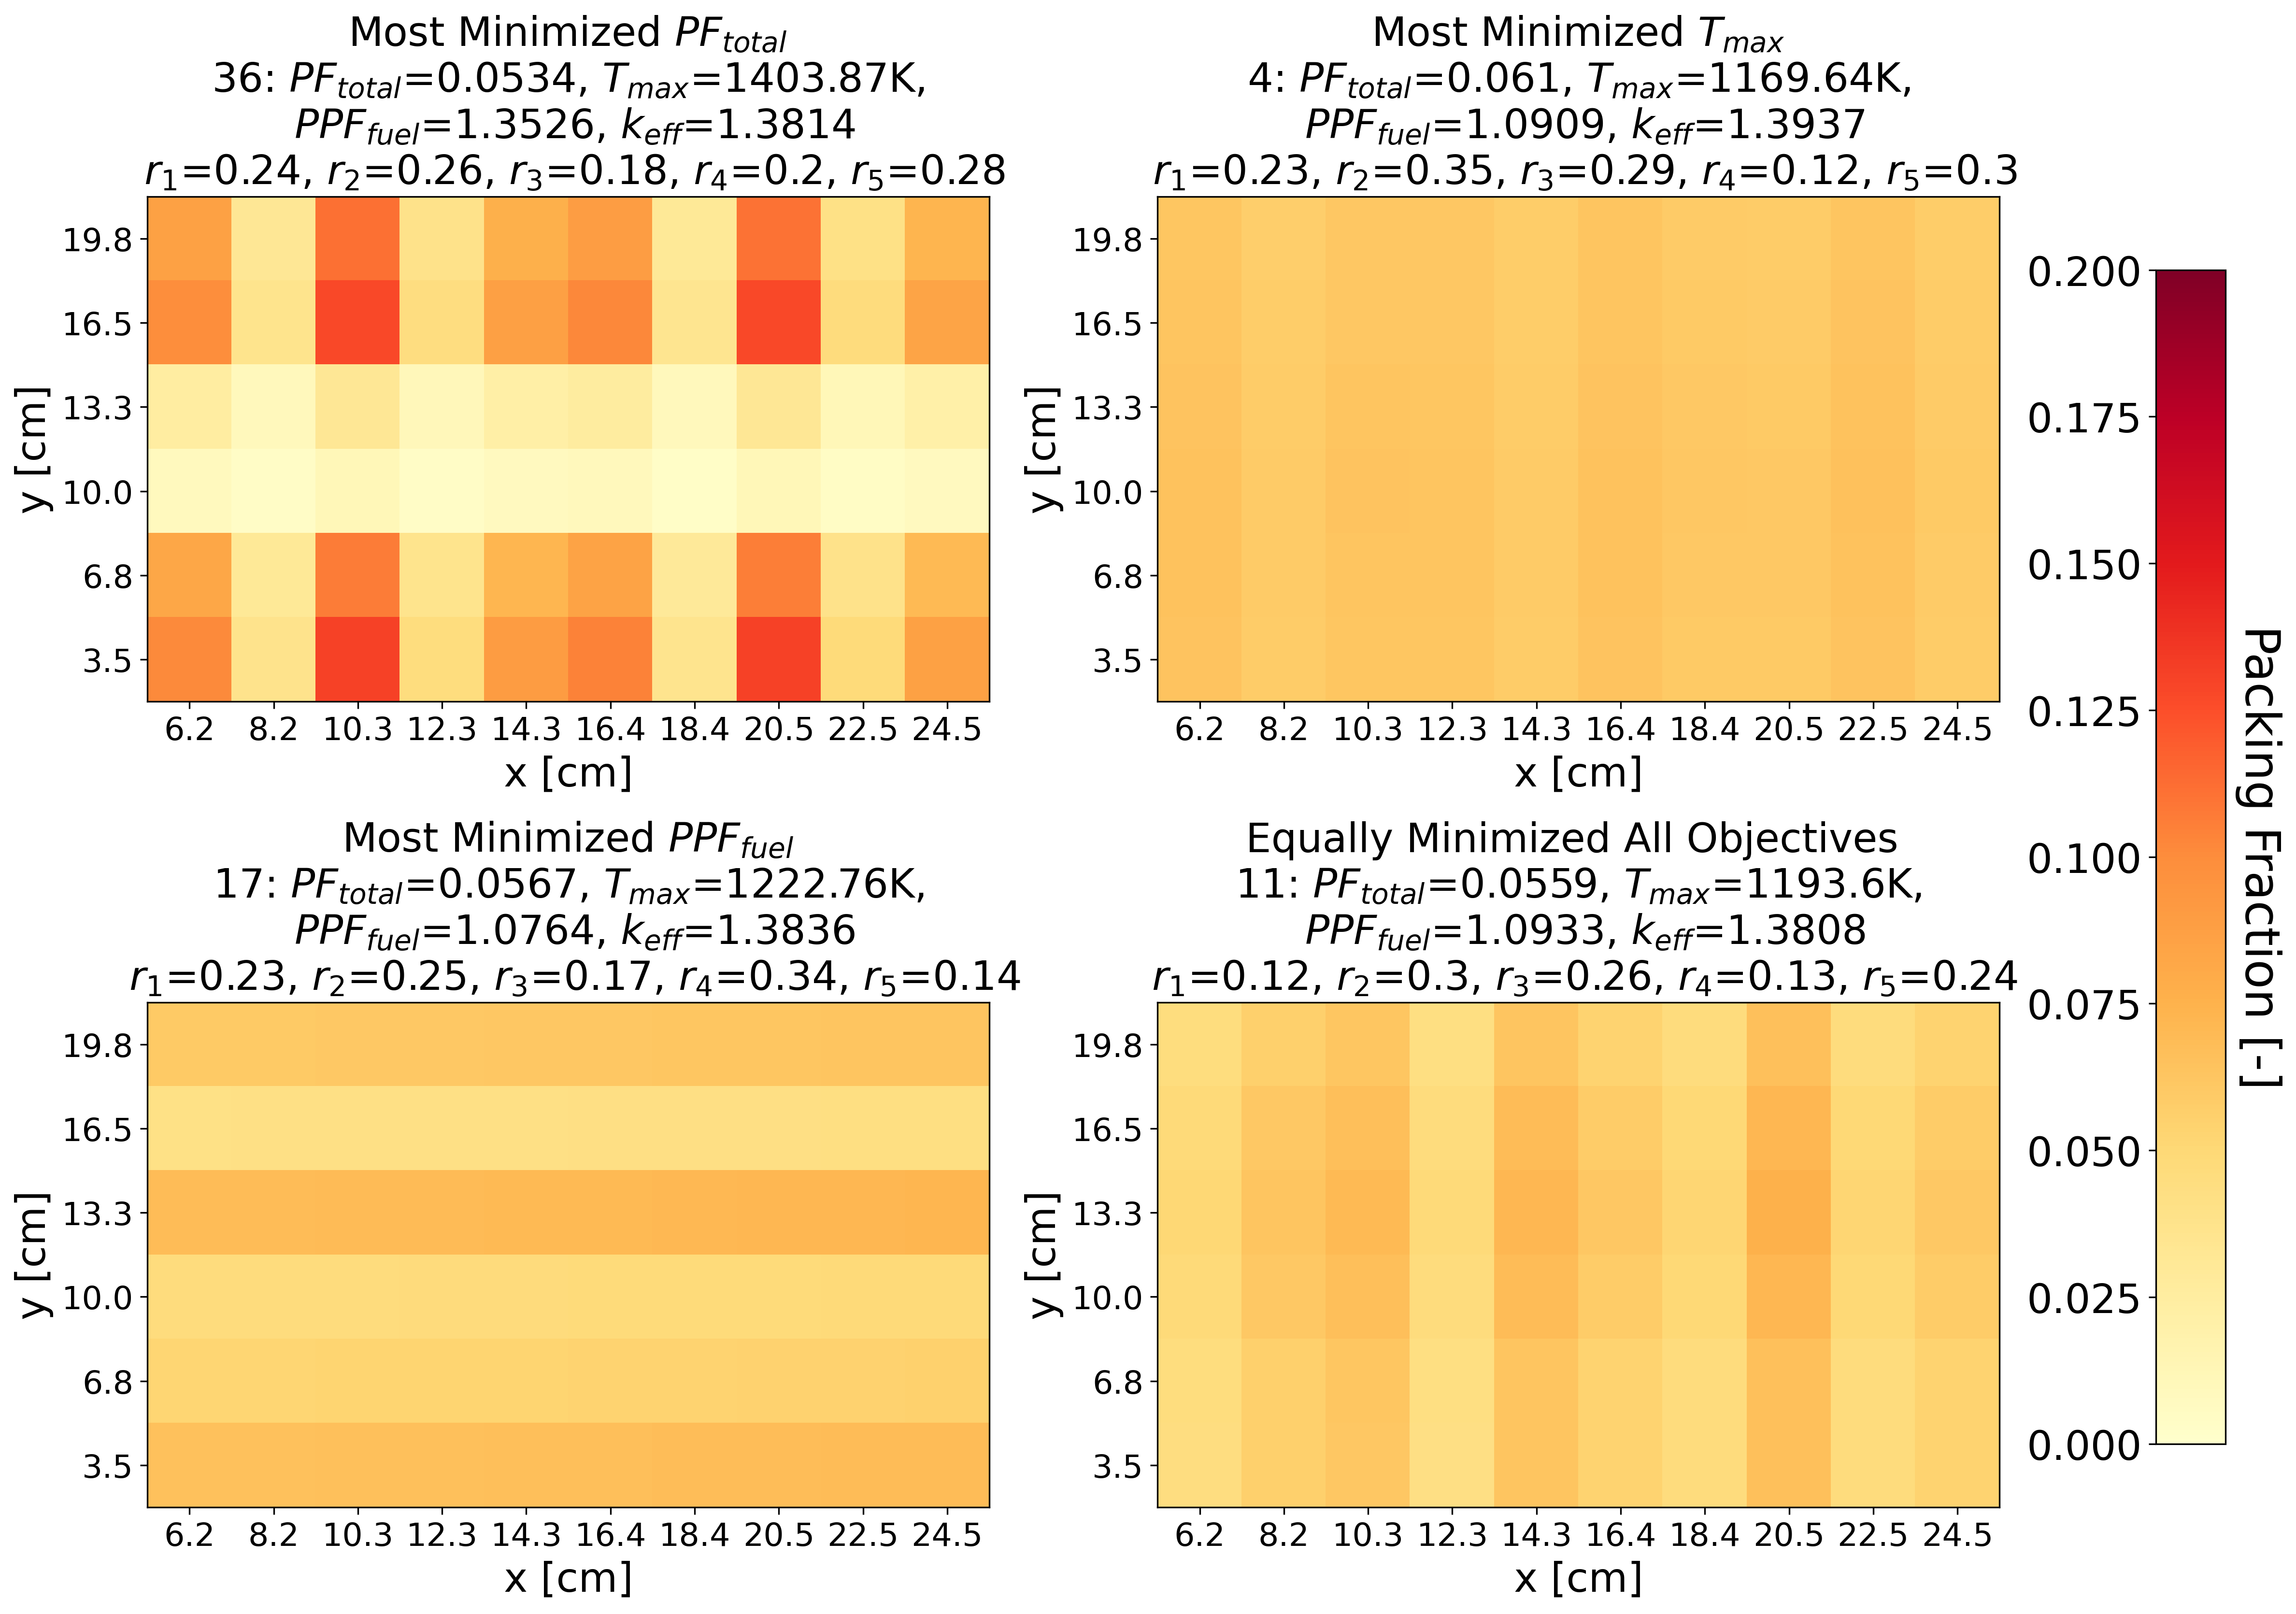
\includegraphics[width=\linewidth]{assem-obj-3-all-256-distr-most-minimized.png}
    \caption{TRISO packing fraction distributions.}
    \label{fig:assem-obj-3-all-256-most-minimized-distr}
    \end{subfigure}
    \caption{AHTR one-third assembly models and TRISO distributions for the 3 reactor 
    models on simulation a-3b-256's Pareto front that most-minimized each objective, and 
    1 reactor model that equally minimized all three objectives.
    Simulation a-3b -- ROLLO triple-objective optimization to minimize 
    total fuel packing fraction ($PF_{total}$), maximum temperature ($T_{max}$), 
    and fuel-normalized power peaking factor ($PPF_{fuel}$) in the one-third assembly. 
    Input parameters varied: total fuel packing fraction $PF_{total}$, 
    TRISO packing fraction distribution ($\rho_{TRISO}(\vec{r})$), 
    coolant channel shape $(r_1, r_2, r_3, r_4, r_5)$.}
    \label{fig:assem-obj-3-all-256-most-minimized}
\end{figure}
\begin{figure}[htbp!]
    \ContinuedFloat
    \begin{subfigure}{0.49\textwidth}
        \centering
        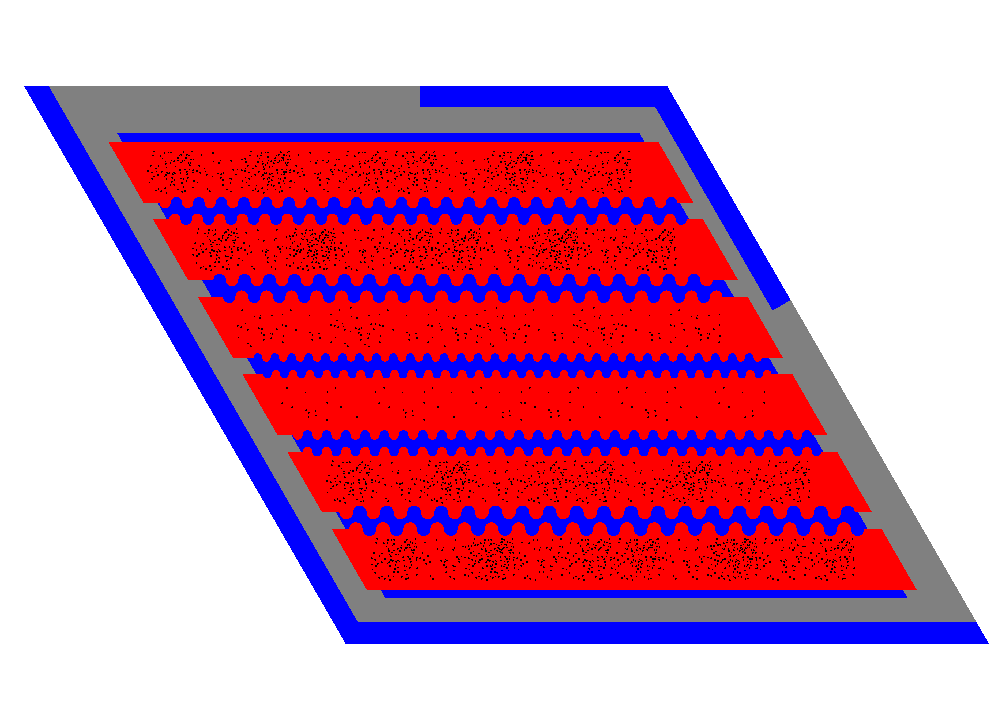
\includegraphics[width=\linewidth]{assem-obj-3-all-256-min-pf.png}
        \caption{\gls{AHTR} one-third assembly model with the most-minimized $PF_{total}$ 
        (reactor model 36).}
        \label{fig:assem-obj-3-all-256-min-pf} 
    \end{subfigure}
    \begin{subfigure}{0.49\textwidth}
        \centering
        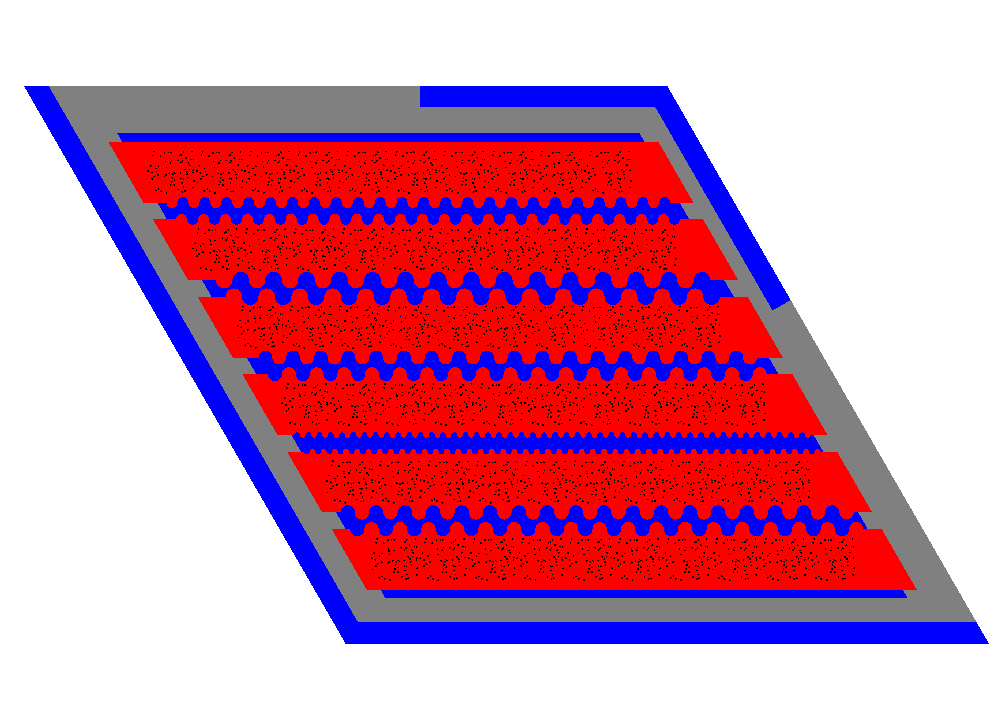
\includegraphics[width=\linewidth]{assem-obj-3-all-256-min-temp.png}
        \caption{\gls{AHTR} one-third assembly model with the most-minimized $T_{max}$
        (reactor model 4).}
        \label{fig:assem-obj-3-all-256-min-temp} 
    \end{subfigure}
    \begin{subfigure}{0.49\textwidth}
        \centering
        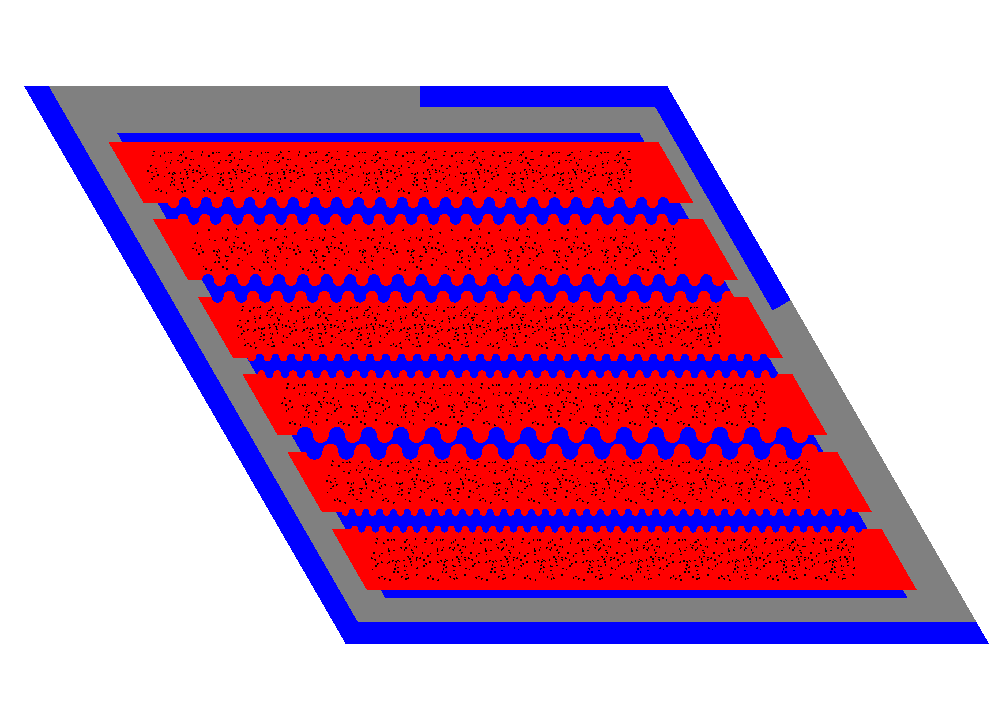
\includegraphics[width=\linewidth]{assem-obj-3-all-256-min-ppf.png}
        \caption{\gls{AHTR} one-third assembly model with the most-minimized $PPF_{fuel}$
        (reactor model 17).}
        \label{fig:assem-obj-3-all-256-min-ppf} 
    \end{subfigure}
    \begin{subfigure}{0.49\textwidth}
        \centering
        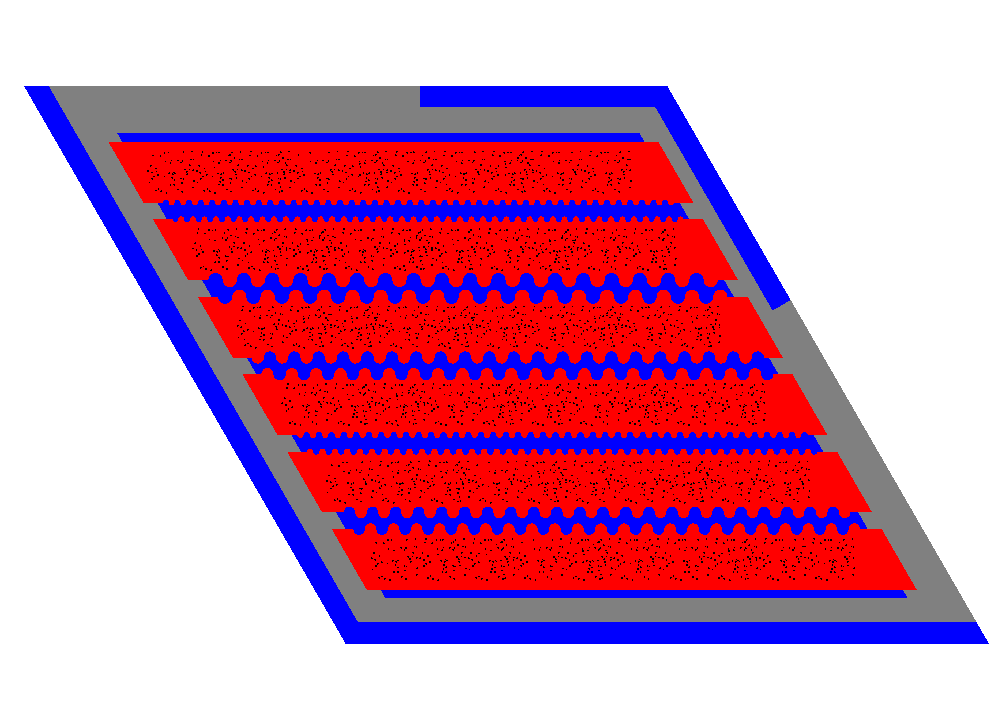
\includegraphics[width=\linewidth]{assem-obj-3-all-256-min-all.png}
        \caption{\gls{AHTR} one-third assembly model that equally minimized all 
        objectives (reactor model 11).}
        \label{fig:assem-obj-3-all-256-min-all} 
    \end{subfigure}
    \begin{subfigure}{.3\textwidth}
    \vspace{1cm}
    \centering
    \resizebox{\textwidth}{!}{
    \fbox{\begin{tabular}{ll}
        \textcolor{fhrblue}{$\blacksquare$} & \gls{FLiBe} \\
        \textcolor{fhrgrey}{$\blacksquare$} & Graphite (Structure)\\
        \textcolor{fhrred}{$\blacksquare$} & Graphite (Fuel Plank) \\
        \textcolor{fhrblack}{$\blacksquare$} & TRISO particle 
        \end{tabular}}}
\end{subfigure}
    \caption{(contd.) AHTR one-third assembly models and TRISO distributions for the 3 reactor 
    models on simulation a-3b-256's Pareto front that most-minimized each objective, and 
    1 reactor model that equally minimized all three objectives.
    Simulation a-3b -- ROLLO triple-objective optimization to minimize 
    total fuel packing fraction ($PF_{total}$), maximum temperature ($T_{max}$), 
    and fuel-normalized power peaking factor ($PPF_{fuel}$) in the one-third assembly. 
    Input parameters varied: total fuel packing fraction $PF_{total}$, 
    TRISO packing fraction distribution ($\rho_{TRISO}(\vec{r})$), 
    coolant channel shape $(r_1, r_2, r_3, r_4, r_5)$.}
\end{figure}

Figure \ref{fig:a-3b-256-temp-distribution} shows the one-third assembly centerline 
temperatures for three reactors on simulation a-3b-356's Pareto front: reactor model 36 
with most-minimized $PF_{total}$, reactor model 4 with most-minimized $T_{max}$, and
reactor model 17 with most-minimized $PPF_{fuel}$.
$r_1$, $r_2$, $r_3$, $r_4$, and $r_5$ values correspond to the FliBe channel at 18cm, 
15cm, 12cm, 8cm, and 6cm, respectively.  
\begin{figure}[htbp!]
    \begin{subfigure}{\textwidth}
        \centering
        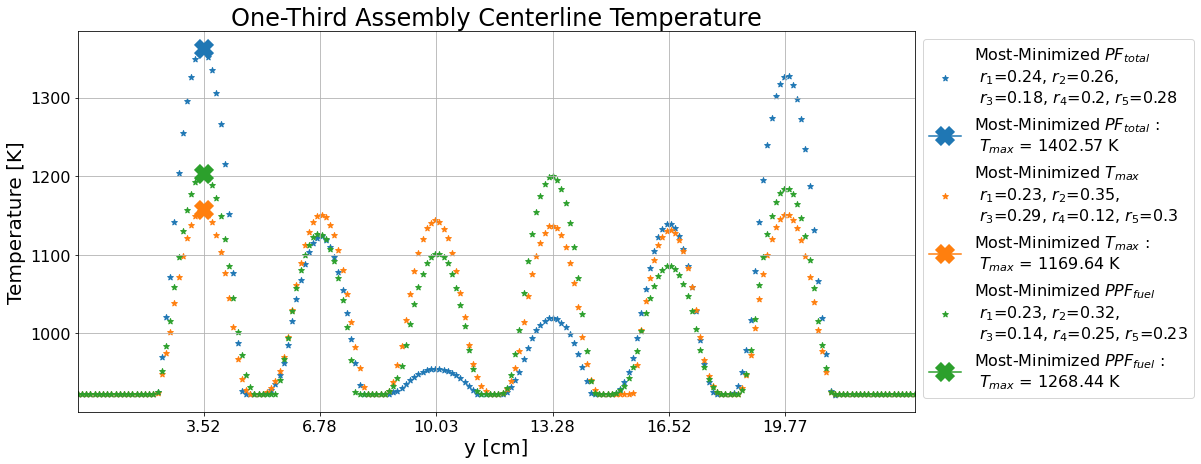
\includegraphics[width=\linewidth]{a-3b-256-centerline-temp.png}
        \caption{Centerline temperature. AHTR assembly's centerline is the white line 
        in Figure \ref{fig:ahtr-assem-verification}.}
        \label{fig:a-3b-256-centerline-temp} 
    \end{subfigure}
    \caption{Simulation a-3b-256's one-third assembly reactor models' temperature 
    distribution. Reactor models are on simulation a-3b-256's Pareto front: 
    reactor model 36 with most-minimized $PF_{total}$, 
    reactor model 4 with most-minimized $T_{max}$, and
    reactor model 17 with most-minimized $PPF_{fuel}$.
    $r_1$, $r_2$, $r_3$, $r_4$, and $r_5$ values correspond to the FliBe channel at 18cm, 
    15cm, 12cm, 8cm, and 6cm, respectively.  }
    \label{fig:a-3b-256-temp-distribution}
\end{figure}
Figure \ref{fig:a-3b-256-centerline-temp} shows that all three reactor models 
peak in the 1st graphite plank (at 3.52cm) with $r_1$ values of ${\sim}0.23cm$. 
The larger radius values closer to temperature peaks enables lower $T_{max}$ values
in simulation a-3b-256 compared to simulation a-3b's equivalent reactor models 
(Figure \ref{fig:a-3b-centerline-temp}). 
This suggests that simulation a-3b-256's larger population size enabled \gls{ROLLO} 
to explore more reactor model variations and find even more optimal reactor models 
that further minimized $T_{max}$. 

The compute time required to run simulation a-3b-256 for 4 generations is 3359 
node-hours. 
Due to the lack of computational resources... 